%%%%%%%% ICML 2025 EXAMPLE LATEX SUBMISSION FILE %%%%%%%%%%%%%%%%%

\documentclass{article}

% Recommended, but optional, packages for figures and better typesetting:
\usepackage{microtype}
\usepackage{graphicx}
\usepackage{subfigure}
\usepackage{booktabs} % for professional tables

% hyperref makes hyperlinks in the resulting PDF.
% If your build breaks (sometimes temporarily if a hyperlink spans a page)
% please comment out the following usepackage line and replace
% \usepackage{icml2025} with \usepackage[nohyperref]{icml2025} above.
\usepackage{hyperref}


% Attempt to make hyperref and algorithmic work together better:
\newcommand{\theHalgorithm}{\arabic{algorithm}}

% Use the following line for the initial blind version submitted for review:
% \usepackage{icml2025}

% If accepted, instead use the following line for the camera-ready submission:
% 保留 [accepted] 以显示真实作者
\usepackage[accepted]{icml2025}
% \usepackage{icml2025}

% For theorems and such
\usepackage{amsmath}
\usepackage{amssymb}
\usepackage{mathtools}
\usepackage{amsthm}

% if you use cleveref..
\usepackage[capitalize,noabbrev]{cleveref}

%%%%%%%%%%%%%%%%%%%%%%%%%%%%%%%%
% THEOREMS
%%%%%%%%%%%%%%%%%%%%%%%%%%%%%%%%
\theoremstyle{plain}
\newtheorem{theorem}{Theorem}[section]
\newtheorem{proposition}[theorem]{Proposition}
\newtheorem{lemma}[theorem]{Lemma}
\newtheorem{corollary}[theorem]{Corollary}
\theoremstyle{definition}
\newtheorem{definition}[theorem]{Definition}
\newtheorem{assumption}[theorem]{Assumption}
\theoremstyle{remark}
\newtheorem{remark}[theorem]{Remark}

% Todonotes is useful during development; simply uncomment the next line
%    and comment out the line below the next line to turn off comments
%\usepackage[disable,textsize=tiny]{todonotes}
\usepackage[textsize=tiny]{todonotes}


% The \icmltitle you define below is probably too long as a header.
% Therefore, a short form for the running title is supplied here:
\icmltitlerunning{Position: The Grounding Gap—From Static Knowledge to Situated Action}

\begin{document}

\twocolumn[
\icmltitle{Position: The Grounding Gap—From Static Knowledge to Situated Action}

% It is OKAY to include author information, even for blind
% submissions: the style file will automatically remove it for you
% unless you've provided the [accepted] option to the icml2025
% package.

% List of affiliations: The first argument should be a (short)
% identifier you will use later to specify author affiliations
% Academic affiliations should list Department, University, City, Region, Country
% Industry affiliations should list Company, City, Region, Country

% You can specify symbols, otherwise they are numbered in order.
% Ideally, you should not use this facility. Affiliations will be numbered
% in order of appearance and this is the preferred way.
% 完全注释掉模板作者机制
% \icmlsetsymbol{equal}{*}
\begin{icmlauthorlist}
\icmlauthor{Yang Liu}{cxmt}
\icmlauthor{Hao Wang}{cxmt}
\icmlauthor{Yanfeng Li}{cxmt}
\icmlauthor{Hongwen Li}{cxmt}
\icmlauthor{Yiming Zhu}{cxmt}
\end{icmlauthorlist}

\icmlaffiliation{cxmt}{Changxin Memory Technologies, Inc. (CXMT)}

\icmlcorrespondingauthor{Yang Liu}{paul.liu@cxmt.com}
\icmlcorrespondingauthor{Yanfeng Li}{yanfeng.li@cxmt.com}
\icmlcorrespondingauthor{Hongwen Li}{howie.li@cxmt.com}

% 手动显示作者
% \vskip 0.15in
% \centerline{\large \textbf{Yang Liu}}
% \vskip 0.05in
% \centerline{\large Independent Researcher}
% \vskip 0.05in
% \centerline{\texttt{foamliu@yeah.net}}
% \vskip 0.25in
]

% this must go after the closing bracket ] following \twocolumn[ ...

% This command actually creates the footnote in the first column
% listing the affiliations and the copyright notice.
% The command takes one argument, which is text to display at the start of the footnote.
% The \icmlEqualContribution command is standard text for equal contribution.
% Remove it (just {}) if you do not need this facility.

\printAffiliationsAndNotice{}  % 显示通讯作者信息


\begin{abstract}
We argue that grounding in dynamic environments requires a runtime architecture for observation and belief update, not just larger models or offline knowledge. LLMs are static compressors of syntax, physical plausibility, and historical facts, but agentic intelligence requires navigating situated states that cannot be learned from text. This grounding gap is structural: frozen parameters contain no guaranteed information about the current state. Bridging it requires an Agent Harness---a runtime architecture supplying observation, belief update, and execution. We formalize this framework via Bayesian inference, show the gap is bounded by observation fidelity rather than model scale, derive three design principles, and validate them empirically on a code-agent benchmark. Our analysis reframes the scaling debate from model capability to system architecture, showing that environmental adaptation comes from observation and action channel design, not parameter tuning.
\end{abstract}
% 中文翻译：
% 我们认为，动态环境中的落地需要一种用于观测和信念更新的运行时架构，而非仅仅依赖更大的模型或离线知识。LLM是语法、物理合理性和历史事实的静态压缩器，但真正的行动智能需要驾驭无法从文本中学习的情境化状态。这一落地鸿沟是结构性的：冻结参数不包含关于当前状态的任何保证信息。弥合它需要智能体框架——一种提供观测、信念更新和执行的运行时架构。我们通过贝叶斯推理形式化该框架，证明鸿沟受观测保真度而非模型规模约束，推导出三条设计原则，并在代码智能体基准上进行了实证验证。我们的分析将规模扩展的讨论从模型能力转向系统架构，表明环境适应来自观测与行动通道设计，而非参数调优。
\section{Introduction}

A striking paradox has emerged in the age of large language models. The same system that passes the bar exam, generates executable code, and proves mathematical theorems can fail catastrophically at tasks a four-year-old performs effortlessly: judging whether a cup is within reach, predicting the outcome of a gentle push, or rerouting around an unexpected obstacle. These are not failures of knowledge---the model likely ``knows'' all the relevant facts. They are failures to translate static knowledge into situated action. An LLM, however capable, is a frozen archive of what has been written. It knows \emph{about} the world, but it does not inhabit it.
% 大语言模型时代出现了一个引人注目的悖论。同一个系统，能通过律师资格考试、生成可执行代码、证明数学定理，却可能在四岁孩童都能轻松完成的任务上灾难性地失败：判断杯子是否在可触及范围内、预测轻轻一推的结果、或绕过意外障碍重新规划路线。这些不是知识的失败——模型很可能"知道"所有相关事实。它们是将静态知识转化为情境化行动的失败。LLM无论多么强大，都只是已书写内容的冻结存档。它"知道"关于世界的事情，但并不栖居于世界之中。

The past two years have witnessed a surge of LLM-based agents that wrap language models with tools, APIs, and memory. Yet despite impressive demos, a pattern of brittleness persists: the web agent fails when a CAPTCHA appears; the robot stalls when an unexpected obstacle blocks its path. This brittleness is not a model problem but a systems problem. The LLM was designed to predict the next token from a static distribution, not to interact with a changing environment. To act, it must be embedded in an external scaffold---an Agent Harness---that supplies observation, execution, and real-time feedback.
% 过去两年间，基于LLM的智能体激增，将语言模型与工具、API和记忆相结合。然而，尽管演示令人印象深刻，脆弱性模式依然存在：验证码出现时网页智能体失败；意外障碍挡住路径时机器人停滞。这种脆弱性不是模型问题而是系统问题。LLM被设计为从静态分布中预测下一个词元，而非与变化的环境交互。要行动，它必须被嵌入一个外部脚手架——智能体框架——以提供观测、执行和实时反馈。

We introduce a four-level hierarchy to make precise what can be learned offline versus what must be observed online. Level 1 (L1), syntactic correctness, concerns well-formedness of symbols. Level 2 (L2), physical plausibility, concerns what events are physically plausible. Level 3 (L3), historical factuality, concerns what has occurred or is documented. These three levels capture regularities learnable from static text. Level 4 (L4), situated truthfulness, is qualitatively different: it concerns what is true \emph{right now}, in this specific environment. L4 is indexical, ephemeral, and requires real-time observation. The gap between L1--L3 and L4 is the \emph{grounding gap}: the structural distance between what a model knows and what an agent must know to act in the present.
% 我们引入一个四层层级来精确区分什么可以离线学习、什么必须在线观测。第一层（L1）语法正确性，关乎符号的形式良好性。第二层（L2）物理合理性，关乎什么事件在物理上是合理的。第三层（L3）历史事实性，关乎什么已经发生或被记录。这三个层次捕捉了可从静态文本中学习的规律性。第四层（L4）情境真实性有质的区别：它关乎"此时此刻"、在这个特定环境中为真的内容。L4是指示性的、瞬时性的，需要实时观测。L1--L3与L4之间的鸿沟就是"落地鸿沟"：模型所知与智能体为在当下行动所必须知道之间的结构性距离。

\textbf{Our central claim is this: L4 knowledge cannot be acquired from static text corpora; frozen parameters contain no L4 information by construction.} Meta-learning is offline generalization over what has been written; it says nothing about online grounding in L4. The Agent Harness bridges this gap: a runtime framework that supplies observation, execution, and feedback. Intelligence emerges from the coupled system of model, harness, and environment, not from the model alone.
% \textbf{我们的核心主张是：L4知识无法从静态文本语料中获得；冻结参数在构造上就不包含L4信息。}元学习是对"已被书写之内容"的离线泛化；它对L4中的在线落地没有说明。智能体框架弥合了这一鸿沟：一个提供观测、执行和反馈的运行时框架。智能涌现自模型、框架和环境耦合的系统，而非模型单独的性质。

We make four contributions. First, we articulate the four-level hierarchy as a diagnostic tool for distinguishing static knowledge from situated state. Second, we formalize grounding using Bayesian inference and distinguish it from inference, simulation, and retrieval. Third, we specify the Agent Harness as an approximate Bayesian decision engine, formalized as \(\mathcal{H} = (\mathcal{S}, \mathcal{O}, \mathcal{A}, \mathcal{B}, \mathcal{T}, \Omega, \Pi)\). Fourth, we derive three architectural principles and validate them empirically on a code-agent benchmark, showing that grounding gains arise from observation fidelity, not model scale. We argue that progress requires shifting investment from bigger models to better harnesses.
% 我们做出四项贡献。第一，阐明四层层级作为区分静态知识与情境状态的诊断工具。第二，使用贝叶斯推理形式化落地，并将其与推理、模拟和检索区分开来。第三，将智能体框架规定为一个近似贝叶斯决策引擎，形式化为\(\mathcal{H} = (\mathcal{S}, \mathcal{O}, \mathcal{A}, \mathcal{B}, \mathcal{T}, \Omega, \Pi)\)。第四，推导三条架构原则，并在代码智能体基准上进行了实证验证，表明落地增益来自观测保真度而非模型规模。我们认为进展需要将投入从更大的模型转向更好的框架。
\section{Related Work}

Our work sits at the intersection of scaling and emergent capabilities, continual learning, LLM-based agents, POMDPs and Bayesian filtering, world models, active perception, and retrieval-augmented systems.
% 我们的工作处于规模扩展与涌现能力、持续学习、基于LLM的智能体、POMDP与贝叶斯滤波、世界模型、主动感知以及检索增强系统的交汇处。

\subsection{LLM Scaling and Emergent Capabilities}

Modern LLMs exhibit emergent abilities at scale---in-context learning, chain-of-thought reasoning, and instruction following \citep{wei2022emergent,brown2020language,schaeffer2023are}. These arise from compressing heterogeneous data under a unified prediction objective. Yet scaling research focuses almost exclusively on training, neglecting deployment in interactive, real-world settings. Scaling improves the prior (L1--L3) but leaves the observational bridge to L4 unaddressed.
% 现代LLM在规模扩大时展现出涌现能力——上下文学习、思维链推理和指令遵循。这些能力源于在统一预测目标下压缩异质数据。然而规模扩展研究几乎完全聚焦于训练，忽略了在交互式真实环境中的部署。规模扩展改善了先验（L1-L3），却未触及通向L4的观测桥梁。

\subsection{Continual Learning}

Modern LLMs epitomize Sutton's paradox: trained once on a fixed corpus, deployed as static artifacts in a continually changing world, unable to learn ``on the job'' \citep{sutton2022plasticity,patel2025sutton}. Our framework responds structurally: decouple knowledge (fixed prior) from belief (dynamic posterior), preserving plasticity at the belief level while avoiding catastrophic forgetting.
% 现代LLM是Sutton悖论的缩影：在固定语料上训练一次，却作为静态制品部署在持续变化的世界中，无法“在工作中学习”。我们的框架提供结构性回应：将知识（固定先验）与信念（动态后验）解耦，在信念层面保持可塑性，同时避免灾难性遗忘。

\subsection{LLM-Based Agents}

LLM-based agents treat the LLM as an orchestrator for decisions, plans, and tool calls \citep{kang2026lifecycle,xie2025empowering}. A recurring observation: LLMs are ``not inherently grounded'' and hallucinate without external evidence \citep{kang2026lifecycle}. Recent work proposes agentic world models bridging planning and physical grounding \citep{zhang2024agentic,ren2026aligning}. However, existing frameworks do not systematically distinguish what an LLM can know from static text (L1--L3) from what it must observe at runtime (L4), nor characterize the bottleneck imposed by observation fidelity. Our work fills this gap with an information-theoretic characterization of grounding and the Agent Harness as a concrete prescription. The critique, however, extends beyond LLMs: any offline-learned prior, whether autoregressive, diffusion-based, or learned simulator, faces the same structural gap.
% 基于LLM的智能体将LLM视为决策、规划和工具调用的编排器。一个反复出现的观察：LLM“本质上没有接地”，没有外部证据时产生幻觉。近期工作提出桥接规划与物理接地的智能体世界模型。然而，现有框架并未系统地区分LLM能从静态文本中知道什么（L1-L3）与它必须在运行时观测什么（L4），也未刻画观测保真度施加的瓶颈。我们的工作通过落地的信息论刻画和Agent Harness作为具体方案填补了这一空白。但这一批判不限于LLM：任何离线学习的先验——无论是自回归、基于扩散的，还是学习到的模拟器——都面临相同的结构性鸿沟。

\subsection{POMDPs, Bayesian Filtering, and Active Perception}

POMDPs provide a mathematical framework for decision-making under uncertainty \citep{kaelbling1998planning,thrun2005probabilistic}. Bayesian filtering---Kalman filters, particle filters---offers principled state estimation from noisy observations \citep{doucet2001sequential}. Active perception treats sensing as part of decision-making \citep{bajcsy1988active,aloimonos1988active}.

Our framework builds on these foundations but differs in purpose. POMDPs formulate the decision problem; we diagnose where the missing information lies architecturally. POMDPs assume well-defined \(\Omega\) and \(\mathcal{T}\); we identify that in LLM-based agents, \(\Omega\) must be supplied by a runtime harness, and its fidelity---not \(\mathcal{T}\)'s capacity---is the bottleneck. We are not solving the POMDP; we are diagnosing why LLM-based agents fail as POMDP solvers.
% POMDP为不确定性下的决策提供了数学框架。贝叶斯滤波——卡尔曼滤波器、粒子滤波器——提供了从噪声观测中进行状态估计的原则性方法。主动感知将感知视为决策的一部分。

% 我们的框架建立在这些基础之上，但目的不同。POMDP形式化了决策问题；我们诊断缺失信息在架构上的位置。POMDP假设良好定义的\(\Omega\)和\(\mathcal{T}\)；我们识别出在基于LLM的智能体中，\(\Omega\)必须由运行时框架提供，其保真度——而非\(\mathcal{T}\)的容量——是瓶颈。我们不是在求解POMDP；我们是在诊断为何基于LLM的智能体无法成为称职的POMDP求解器。

\subsection{World Models and Learned Priors}

World models---learned simulators of environment dynamics---have been explored in robotics and RL \citep{ha2018world,lecun2022pathways,schmidhuber1990making}. Recent agentic world models incorporate LLMs \citep{zhang2024agentic,ren2026aligning}.

Our framework distinguishes two roles of a world model. Offline, it encodes L1--L3 general regularities. At runtime, the agent must condition this prior on L4 observations. The transition kernel \(\mathcal{T}\) abstracts the world model's prior role, not predictive accuracy. The key limitation: even a perfect world model, frozen at deployment, cannot provide L4 information about the current state---that requires observation. The fidelity of \(\Omega\), not the expressiveness of the world model, is the binding constraint.
% 世界模型——环境动态的学习模拟器——已在机器人和RL中被广泛探索。最近的智能体世界模型将LLM纳入其中。

% 我们的框架区分了世界模型的两个角色。离线时，它编码L1-L3的一般规律性。运行时，智能体必须将此先验条件化于L4观测之上。转移核\(\mathcal{T}\)抽象了世界模型的先验角色，而非预测准确性。关键限制：即使完美的世界模型，在部署时冻结，也无法提供当前状态的L4信息——这需要观测。\(\Omega\)的保真度，而非世界模型的表达能力，是约束性瓶颈。

\subsection{Grounding, Retrieval, and Memory}

A common confusion equates grounding with retrieval or memory. Retrieval-augmented generation (RAG) retrieves from external datastores \citep{lewis2020retrieval,gao2023retrieval}. Memory stores past experiences \citep{zhong2024memory}. Both are valuable, but neither is grounding. Retrieval queries the past; memory recalls the past. Grounding is the process of bringing offline knowledge into contact with \emph{current} L4 states. An agent with perfect retrieval and infinite memory still cannot know whether the cup is on the table \emph{now} unless it observes. This distinction---recalling what was versus observing what is---is our central contribution.
% 一个常见混淆是将接地等同于检索或记忆。检索增强生成（RAG）从外部存储检索。记忆存储过去的经验。两者都有价值，但都不是接地。检索查询过去；记忆回忆过去。接地是将离线知识与\emph{当前}L4状态相接触的过程。一个拥有完美检索和无限记忆的智能体，除非观测，否则仍然无法知道杯子此刻是否在桌上。这一区分——回忆曾经是什么与观测当前是什么——是我们的核心贡献。
\section{The Four Levels of Information}

We introduce a four-level distinction that separates what can be acquired offline from what must be observed online. The distinction applies to any agent that must act after its knowledge has been fixed through offline learning: \emph{generalized prior knowledge} acquirable before deployment versus \emph{situated state information} that depends on the specific environment at a specific time.
% 我们引入一个四层区分，将可以离线获取的内容与必须在线观测的内容分开。该区分适用于任何必须在知识通过离线学习固定后行动的智能体：部署前可获取的"泛化先验知识"与依赖于特定时间具体环境的"情境状态信息"。

\textbf{Level 1 (L1) -- Syntactic Correctness.} Well-formedness of symbols according to formal rules. Captured by formal grammars and the syntactic capacities of modern LLMs.
% 第一层（L1）——语法正确性。符号根据形式规则的形式良好性。由形式语法和现代LLM的句法能力所覆盖。

\textbf{Level 2 (L2) -- Physical Plausibility.} What events are physically plausible or generally expected: objects do not pass through walls, water flows downhill. L2 captures robust statistical patterns of the physical world, not logical certainties. These regularities are general and can be acquired through offline learning, constituting the agent's \emph{prior} over how the world typically behaves.
% 第二层（L2）——物理合理性。什么事件在物理上是合理的或普遍可预期的：物体不会穿过墙壁，水往低处流。L2捕捉物理世界的稳健统计模式，而非逻辑确定性。这些规律性是一般的，可以通过离线学习获得，构成智能体关于世界通常如何运作的\emph{先验}。

\textbf{Level 3 (L3) -- Historical Factuality.} What has actually occurred or is documented as fact: Paris is the capital of France. L3 concerns actual rather than merely possible states of affairs. Like L1 and L2, L3 can be acquired offline, but it is past-oriented, describing what was true as of the training cutoff, with no connection to what is true \emph{now}.
% 第三层（L3）——历史事实性。什么已经实际发生或被记录为事实：巴黎是法国的首都。L3关乎"实际的"而非仅仅是"可能的"事态。与L1和L2一样，L3可以离线获取，但它是面向过去的，描述截至训练截止日期为真的内容，与"此刻"为真的内容没有联系。

\textbf{Level 4 (L4) -- Situated Truthfulness.} L4 is qualitatively different. It concerns what is true \emph{right now}, in this specific environment. Three characteristics define it: (1) \emph{indexicality}---truth depends on context and changes over time; (2) \emph{non-guaranteeability from offline data}---no offline dataset can \emph{guarantee} the current L4 state, though it may induce strong priors; (3) \emph{real-time commitment}---L4 knowledge must be acquired continuously and acted upon promptly. To know L4, a system must observe its environment at runtime.
% 第四层（L4）——情境真实性。L4有质的区别。它关乎"此时此刻"、在这个特定环境中为真的内容。三个特征定义它：（1）指示性——真值依赖于语境并随时间变化；（2）无法从离线数据获得保证——没有离线数据集能保证当前的L4状态，尽管它可以诱导出强先验；（3）实时承诺——L4知识必须被持续获取并迅速据此行动。要知晓L4，系统必须在运行时观测其环境。

These four levels are ordered by their dependence on runtime access. Critically, L4 is not a semantic category of propositions; it is a \emph{grounding requirement} imposed by indexical reference. The same proposition may be L3 at one time and L4 at another, depending on whether it refers to a past fact or a current state. \textbf{L4 cannot be guaranteed by a frozen representation of the environment alone.} This is the core of the grounding gap.
% 这四个层次按其运行时依赖程度排序。关键在于，L4不是命题的语义类别；它是由指示性所指强加的\emph{落地要求}。同一个命题可能在某个时刻是L3，在另一个时刻是L4，取决于它指的是过去的事实还是当前的状态。\textbf{L4无法仅靠环境的冻结表征来保证。}这就是落地鸿沟的核心。

\subsection{Why L4 Cannot Come from Offline Knowledge}

The four-level distinction explains why systems built from offline learning cannot perform grounding natively without runtime observation. This is not to deny that offline learning can induce strong priors over L4---such priors are valuable---but priors are not observations, and guessing is not grounding. Four architectural consequences follow from L4's defining characteristics:
% 四层区分解释了为什么从离线学习构建的系统在没有运行时观测的情况下无法原生执行落地。这并非否认离线学习可以诱导出关于L4的强先验——这样的先验是有价值的——但先验不是观测，猜测不是落地。从L4的定义性特征可以推出四个架构性后果：

\begin{enumerate}
\item \emph{No observation modules}: L4 requires real-time observation; offline-trained systems have no native sensors beyond training inputs.
% 无观测模块：L4需要实时观测；离线训练的系统除了训练输入外没有原生传感器。

\item \emph{No persistent situated state}: L4 is indexical and time-dependent. Frozen deployment does not maintain an environment-grounded belief state across time.
% 无持久情境状态：L4是指示性的、时间依赖的。冻结部署不跨时间维护基于环境的信念状态。

\item \emph{No execution interface}: L4 requires action; prediction-only systems have no native effectors.
% 无执行接口：L4需要行动；仅预测的系统没有原生执行器。

\item \emph{No real-time feedback loop}: L4 requires continuous updating; frozen systems receive no feedback about output consequences.
% 无实时反馈环路：L4需要持续更新；冻结系统不接收关于输出后果的反馈。
\end{enumerate}

These are not incidental shortcomings; they are consequences of offline training's fundamental design. Every observed failure of LLM-based agents in dynamic environments traces to one or more of these missing components.
% 这些不是偶发缺陷；它们是离线训练基本设计的后果。基于LLM的智能体在动态环境中的每一个观察到的失败都可追溯到一个或多个这些缺失的组件。

\subsection{The Situated State Is Not Limited to Physics}

The situated state \(\theta_t\) is not limited to the physical world. It encompasses any aspect of the environment that is (a) temporally indexed, (b) context-dependent, and (c) not fully determined by static knowledge: digital states (DOM, repository status), informational states (market data, unread emails), and social states (a user's current intent). The grounding problem is isomorphic across these domains: the agent must observe the current state through a domain-specific runtime channel. L4 is whatever must be \emph{read} from the environment rather than \emph{recalled} from memory. This holds regardless of modality---whether L4 arrives as text, pixels, or sensor readings, it must be acquired at runtime, not recalled from frozen parameters.
% 情境状态\(\theta_t\)不限于物理世界。它涵盖环境中任何（a）具有时间索引的、（b）依赖于上下文的、（c）不能被静态知识完全确定的方面：数字状态（DOM、仓库状态）、信息状态（市场数据、未读邮件）和社会状态（用户的当前意图）。落地问题在这些领域中是同构的：智能体必须通过特定领域的运行时通道观测当前状态。L4是必须从环境中"读取"而非从记忆中"回忆"的任何东西。无论何种模态——无论L4以文本、像素还是传感器读数形式到来——它都必须在运行时被获取，而非从冻结参数中回忆。

This is not a claim that LLMs cannot \emph{access} L4 via tools or APIs. It is a claim about the \emph{source}: L4 must enter through runtime observation, not pretraining. A weather API supplies today's temperature; the LLM interprets it, but the observation itself comes from the environment.
% 这并不是说LLM不能通过工具或API"访问"L4。这是关于信息"来源"的主张：L4必须通过运行时观测进入系统，而非预训练。天气API提供今天的温度；LLM解释它，但观测本身来自环境。

The four-level distinction is not a taxonomy of all knowledge. It distinguishes what can be \emph{known in advance} from what must be \emph{observed now}. L4 is the only level that systematically resists offline encoding, requiring a fundamentally different mode of engagement with the world.
% 四层区分并非所有知识的分类法。它区分了什么可以"预先知道"与什么必须"此刻观测"。L4是唯一系统性地抵抗离线编码的层次，需要一种根本不同的与世界互动的方式。

\begin{table*}[t]
\centering
\caption{The four levels of information.}
\label{tab:hierarchy}
\small
\setlength{\tabcolsep}{3pt}
\begin{tabular}{c p{3.5cm} p{3.8cm} c}
\toprule
\textbf{Level} & \textbf{Name} & \textbf{Core Question} & \textbf{Learnable Offline?} \\
\midrule
L1 & Syntactic Correctness & Is this string well-formed? & Yes \\
L2 & Physical Plausibility & Could this event happen? & Yes \\
L3 & Historical Factuality & Did this event happen? & Yes \\
L4 & Situated Truthfulness & Is this true \emph{right now}? & \textbf{No} \\
\bottomrule
\end{tabular}
\end{table*}
% 中文翻译：表格内容同上，已省略
\section{Grounding: Bridging Knowledge and Action}

We define \emph{grounding} as the process by which offline knowledge (L1--L3) is brought into contact with situated states (L4), enabling an agent to act effectively in the here and now. Grounding is temporal (real-time), causal (terminates in action, not representation), and iterative (action results feed back into observation). It is not inference, simulation, retrieval, or translation---all of which remain within the offline or symbolic domain.
% 我们将"落地"定义为将离线知识（L1-L3）与情境状态（L4）相接触的过程，使智能体能够在此时此地有效地行动。落地是时间性的（实时）、因果性的（终止于行动而非表征）和迭代性的（行动结果反馈到观测）。它不是推理、模拟、检索或翻译——这些都停留在离线或符号领域。

\subsection{The Grounding Gap}

The grounding gap is the distance between what a model knows from offline learning (L1--L3) and what an agent must observe to act in the present (L4). This gap is structural---any architecture that freezes knowledge before deployment suffers it. Offline data and scaling improve only the prior, not the observation of L4. Prediction from the prior cannot replace observation of what the state \emph{is}; they are epistemically distinct operations.
% 落地鸿沟是模型从离线学习中所知（L1-L3）与智能体为在当下行动所必须观测（L4）之间的距离。这一鸿沟是结构性的——任何在部署前冻结知识的架构都受其影响。离线数据和规模扩展只改善先验，而非L4的观测。从先验预测无法替代对状态"实际"是什么的观测；二者在认识论上是不同的操作。

\subsection{A Bayesian Formalization of Grounding}

The Bayesian formulation that follows is \emph{diagnostic, not algorithmic}. It is not a blueprint for tractable inference---which is intractable in high-dimensional \(\mathcal{S}\)---but a normative standard that makes precise \emph{what} is missing: the observation likelihood \(\Omega\) and the recursive update \(\Phi\). This mirrors the role of POMDPs in robotics: few systems solve them exactly, yet the formalism clarifies where information is lost.
% 以下贝叶斯形式化是"诊断性"的，而非"算法性"的。它不是高维\(\mathcal{S}\)中可处理推理的蓝图——那本身是不可处理的——而是一个规范性标准，精确指明"什么"是缺失的：观测似然\(\Omega\)和递归更新\(\Phi\)。这镜像了POMDP在机器人学中的角色：很少有系统精确求解它们，但形式化框架阐明了信息在何处丢失。

Let \(\Theta\) be the space of L4 states, \(o_t\) the observation, \(a_t\) the action, and \(\mathcal{K}\) offline knowledge. The agent's belief about the current L4 state is:
% 令\(\Theta\)为L4状态空间，\(o_t\)为观测，\(a_t\)为行动，\(\mathcal{K}\)为离线知识。智能体对当前L4状态的信念为：

\begin{equation}
b_t(\theta) \triangleq p(\theta_t \mid o_{1:t}, a_{1:t-1}, \mathcal{K})
\end{equation}

updated via Bayes' rule:
% 通过贝叶斯法则更新：

\begin{equation}
b_t(\theta) \propto p(o_t \mid \theta_t, \mathcal{K}) \int p(\theta_t \mid \theta_{t-1}, a_{t-1}, \mathcal{K}) \, b_{t-1}(\theta_{t-1}) \, d\theta_{t-1}
\end{equation}

where \(p(o_t \mid \theta_t, \mathcal{K})\) is the observation likelihood and \(p(\theta_t \mid \theta_{t-1}, a_{t-1}, \mathcal{K})\) is the transition model. Actions are selected by minimizing expected cost:
% 其中\(p(o_t \mid \theta_t, \mathcal{K})\)是观测似然，\(p(\theta_t \mid \theta_{t-1}, a_{t-1}, \mathcal{K})\)是转移模型。行动通过最小化期望代价选择：

\begin{equation}
a_t^* = \arg\min_{a \in \mathcal{A}} \; \mathbb{E}_{\theta_t \sim b_t}\left[ \mathcal{C}(\theta_t, a, G) + \gamma \, V(b_{t+1}) \right]
\end{equation}

The grounding gap is the divergence between the posterior with runtime observations and the posterior from the offline prior alone:
% 落地鸿沟是融合运行时观测的后验与仅依赖离线先验的后验之间的散度：

\begin{equation}
D_{\text{grounding}}(t) \triangleq D_{\text{KL}}\left(p(\cdot \mid o_{1:t}, \mathcal{K}, \text{env}) \;\middle\|\; p_{\mathcal{K}}(\cdot \mid o_{1:t})\right)
\end{equation}

This formulation is \emph{conceptual}, not implementable. It makes precise why L4 requires runtime observation---\(\Omega\) is irreducible to \(\mathcal{K}\)---and reveals the bottleneck: observation fidelity, not model scale. If \(I(\Theta_t; O_t \mid \mathcal{K}) = 0\), no prior improvement can recover the current state. The observation channel is the binding constraint.
% 这一形式化是"概念性"的，而非可实现的。它精确说明了为什么L4需要运行时观测——\(\Omega\)不可还原为\(\mathcal{K}\)——并揭示了瓶颈：观测保真度，而非模型规模。如果\(I(\Theta_t; O_t \mid \mathcal{K}) = 0\)，再多的先验改进也无法恢复当前状态。观测通道是约束性瓶颈。

\subsection{The Source of the Gap Is Causal, Not Statistical}

The grounding gap is causal, not merely statistical. Parameters are fixed before deployment; facts that come into existence after the training cutoff---or states that depend on unrepeatable circumstances---cannot be present in the parameters by definition. The environment at time \(t\) is not a function of the training corpus. Offline data and scaling affect only the prior, not the availability of runtime observation.
% 落地鸿沟的来源是因果性的，而不仅仅是统计性的。参数在部署前固定；训练截止后产生的事实——或依赖于不可重复情境的状态——在定义上不可能存在于参数中。\(t\)时刻的环境不是训练语料的函数。离线数据和规模扩展只影响先验，不影响运行时观测的可得性。

\subsection{Grounding vs. Meta-Learning}

Meta-learning is a capability acquired during \emph{training}: the model learns to learn over L1--L3 distributions, improving the \emph{prior}. Grounding occurs during \emph{deployment}: it requires the \emph{likelihood} and posterior update from observing \(o_t\). A better prior does not eliminate the need for observation. They are complementary---one offline, one online; one about knowledge, one about belief. Scaling improves the prior; grounding improves the likelihood.

In-context learning (ICL) offers a nuanced intermediate case: it updates the model's behavior in response to recent observations without modifying parameters, operating in activation space rather than structured state space. ICL can serve as a fast, approximate surrogate for \(\Phi\) in low-uncertainty regimes, but it maintains no explicit posterior \(b_t(\theta)\), no uncertainty quantification, and no principled mechanism for filtering stale context. The two mechanisms are complementary, not competing: ICL provides rapid contextual adaptation; \(\Phi\) provides principled state estimation. Future harness designs may productively integrate both.
% 上下文学习（ICL）提供了一个微妙的中间情况：它在不修改参数的情况下，根据最近的观测更新模型行为，运作在激活空间而非结构化状态空间中。ICL可以作为低不确定性情境下\(\Phi\)的快速近似替代，但它不维护显式的后验\(b_t(\theta)\)，没有不确定性量化，也没有过滤过时上下文的原理性机制。这两种机制是互补而非竞争的：ICL提供快速上下文适应；\(\Phi\)提供原理性的状态估计。未来的框架设计可以有效地整合两者。
% \section{The Agent Harness: Enacting Grounding}

The Agent Harness is the runtime architecture that bridges the LLM's frozen prior (\(\mathcal{K}\), L1--L3) with real-time L4 states. It supplies what the LLM lacks: observation, belief update, and execution. The LLM provides the prior and approximates planning; the Harness closes the loop. Grounding is an emergent property of the coupled system, not of the model alone.
% 智能体框架是连接LLM冻结先验（\(\mathcal{K}\)，L1-L3）与实时L4状态的运行时架构。它提供了LLM所缺乏的：观测、信念更新和执行。LLM提供先验并近似规划；框架闭合环路。落地是耦合系统的涌现属性，而非模型单独的性质。

\begin{figure*}[t]
    \centering
    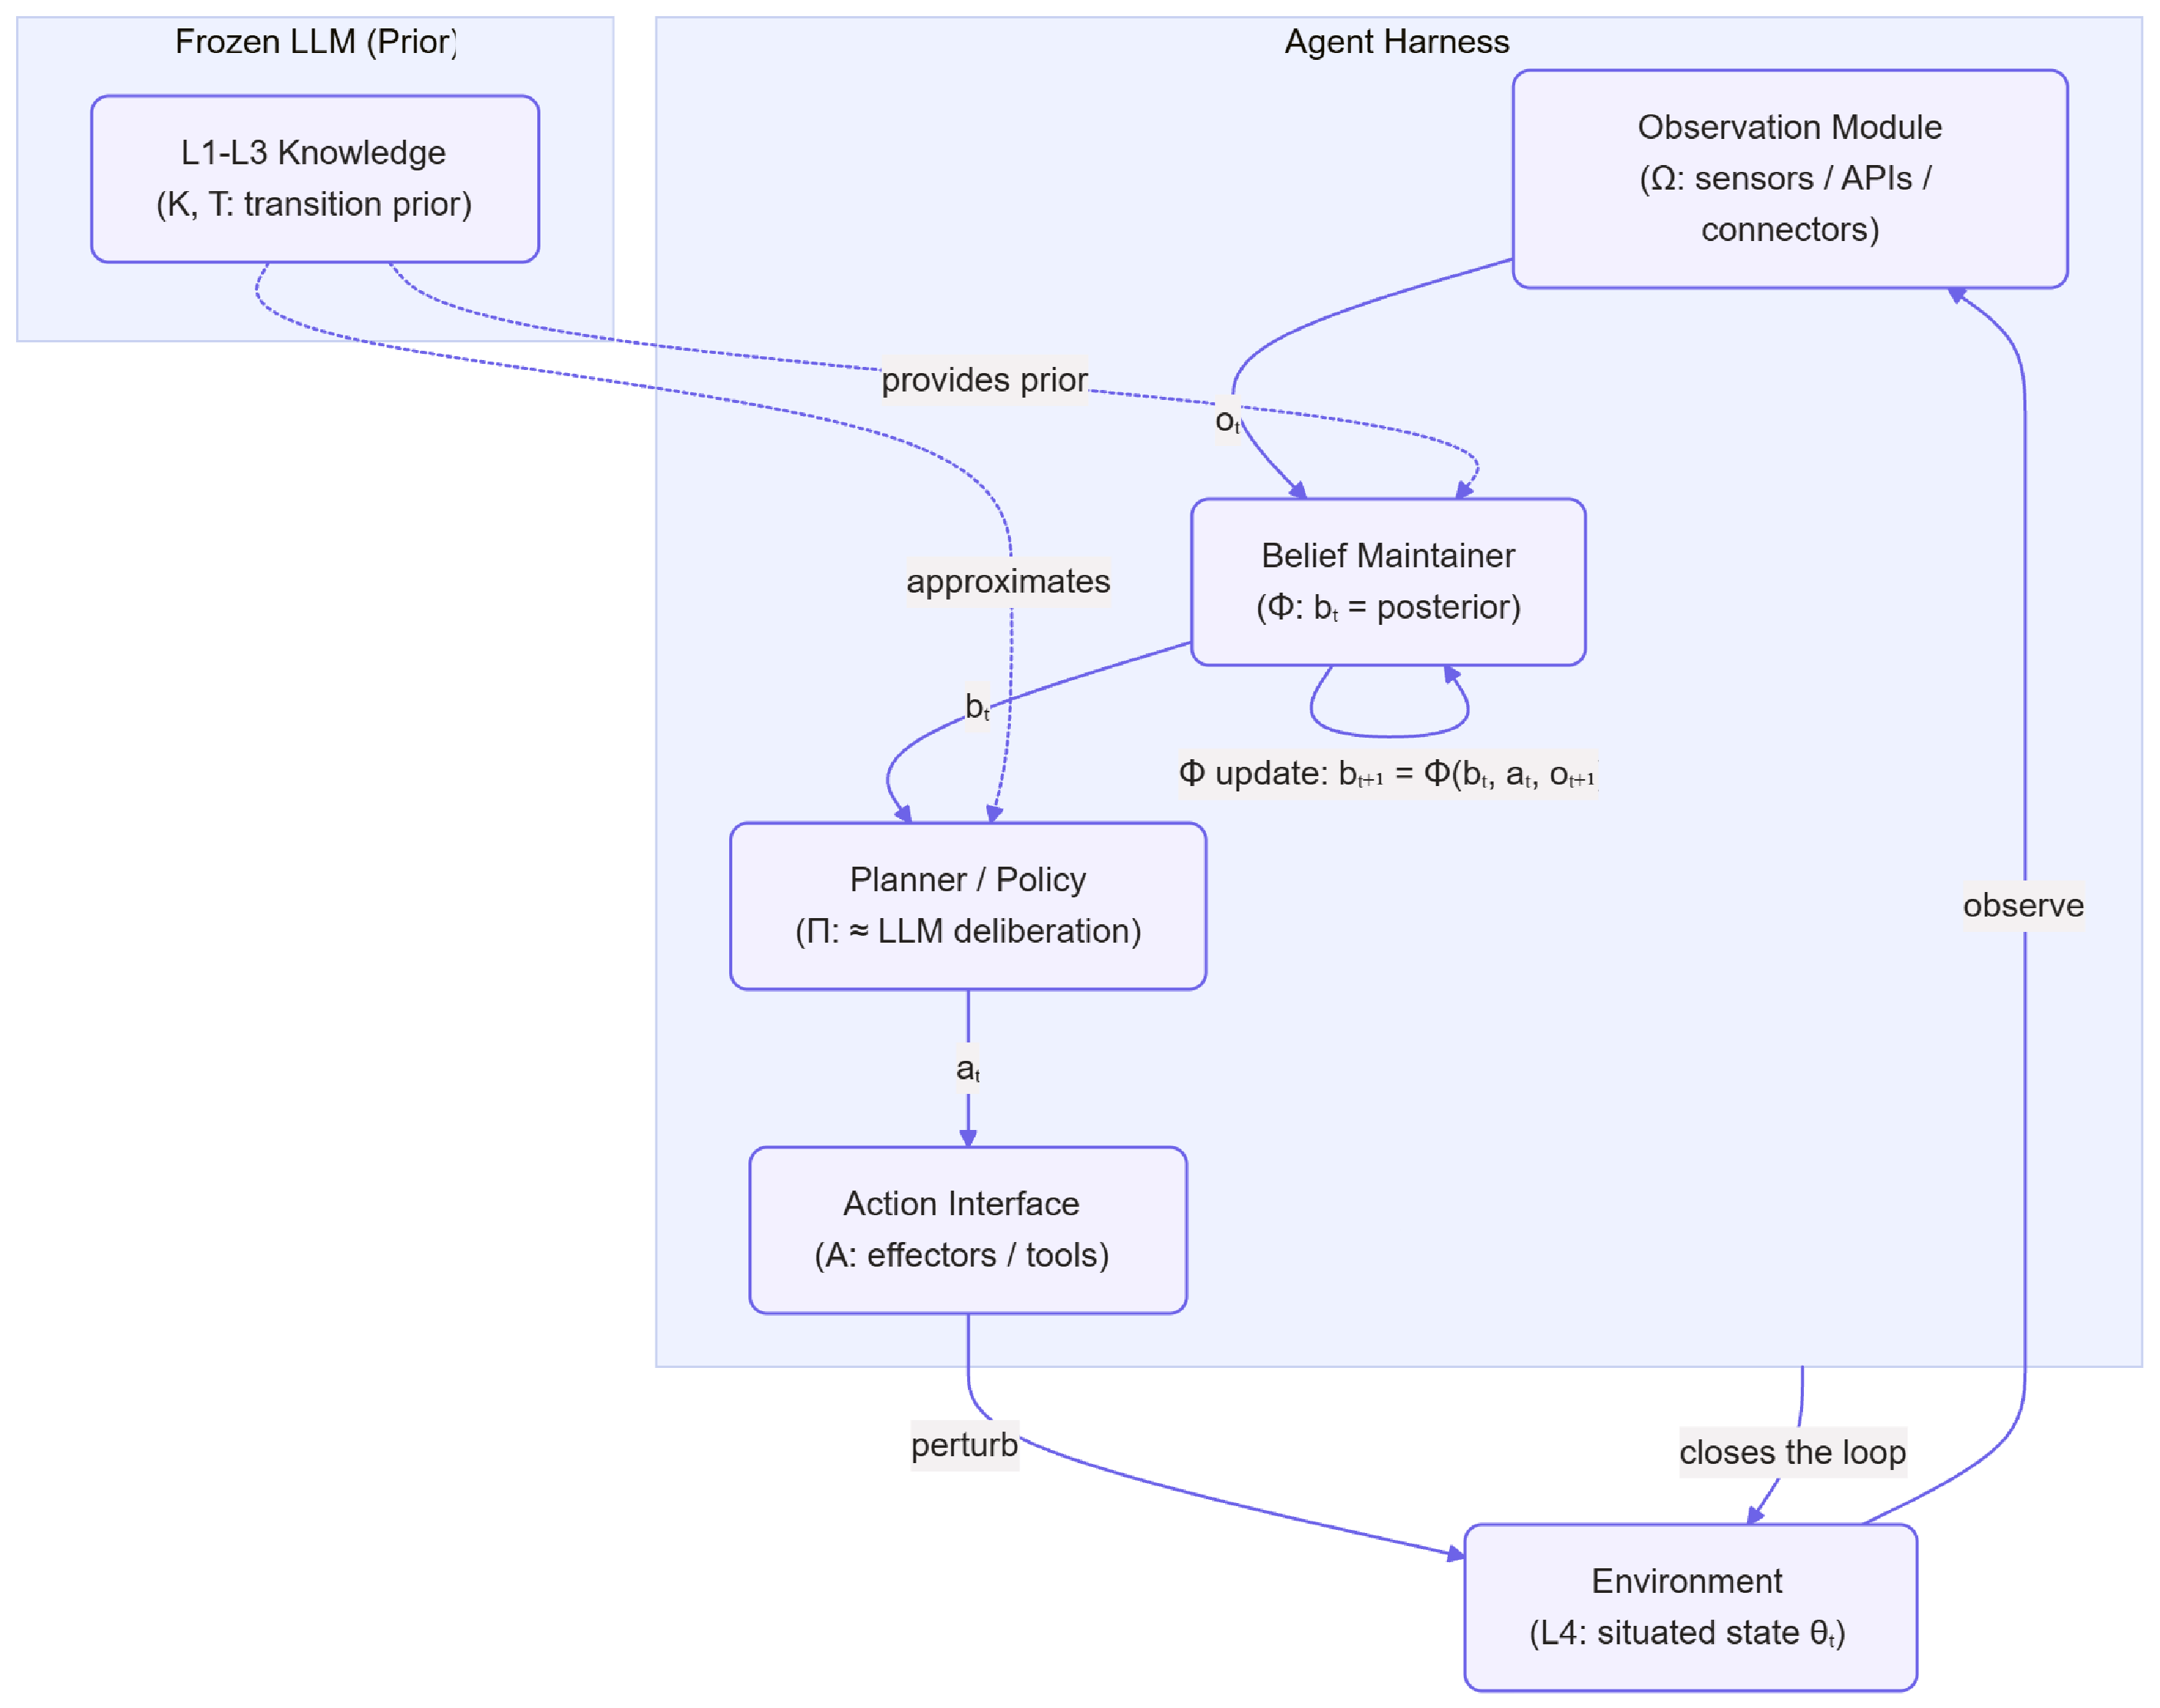
\includegraphics[width=0.85\textwidth]{figures/harness-architecture.pdf}
    \caption{The Agent Harness architecture. The frozen LLM provides \(\mathcal{K}\) and \(\mathcal{T}\); the Harness supplies \(\Omega\), \(\Phi\), and \(\Pi\). Solid arrows: data flow; dashed arrows: prior provision.}
    \label{fig:harness}
\end{figure*}
% 图：智能体框架架构。冻结LLM提供\(\mathcal{K}\)和\(\mathcal{T}\)；框架提供\(\Omega\)、\(\Phi\)和\(\Pi\)。实线箭头：数据流；虚线箭头：先验供给。

\subsection{Formalizing the Harness Architecture}

The Harness is a tuple:
\begin{equation}
\mathcal{H} = (\mathcal{S}, \mathcal{O}, \mathcal{A}, \mathcal{B}, \mathcal{T}, \Omega, \Pi),
\end{equation}
where each component corresponds to a concrete computational module:
% 框架定义为一个七元组，每个组件对应一个具体的计算模块：

\begin{itemize}
\item \(\mathcal{S} \subseteq \mathbb{R}^n\): the space of L4 environmental states \(\theta_t\), acted upon through effectors but not observed directly.
% \(\mathcal{S} \subseteq \mathbb{R}^n\)：L4环境状态\(\theta_t\)的空间，通过执行器作用于其上，但不直接观测。

\item \(\mathcal{O} \subseteq \mathbb{R}^m\): the observation space, comprising all possible observations \(o_t\) from observation modules.
% \(\mathcal{O} \subseteq \mathbb{R}^m\)：观测空间，包含来自观测模块的所有可能观测\(o_t\)。

\item \(\mathcal{A} \subseteq \mathbb{R}^k\): the action space available to the agent, instantiated through effectors.
% \(\mathcal{A} \subseteq \mathbb{R}^k\)：智能体可用的动作空间，通过执行器实例化。

\item \(\mathcal{B} \subseteq \Delta(\mathcal{S})\): the belief space, where \(b_t(\theta) = p(\theta_t \mid o_{1:t}, a_{1:t-1}, \mathcal{K})\) is the maintained posterior over L4 states.
% \(\mathcal{B} \subseteq \Delta(\mathcal{S})\)：信念空间，其中\(b_t(\theta) = p(\theta_t \mid o_{1:t}, a_{1:t-1}, \mathcal{K})\)是维护的L4状态后验。

\item \(\mathcal{T}: \mathcal{S} \times \mathcal{A} \to \Delta(\mathcal{S})\): the transition kernel
\begin{equation}
\mathcal{T}(\theta_{t+1} \mid \theta_t, a_t) = p(\theta_{t+1} \mid \theta_t, a_t, \mathcal{K}),
\end{equation}
representing the LLM's learned prior over dynamics---an abstraction, not a ground-truth function.
% \(\mathcal{T}: \mathcal{S} \times \mathcal{A} \to \Delta(\mathcal{S})\)：转移核，表示LLM学习的动态先验——是一个抽象，而非真实函数。

\item \(\Omega: \mathcal{S} \to \Delta(\mathcal{O})\): the observation likelihood
\begin{equation}
\Omega(o_t \mid \theta_t) = \tilde{p}(o_t \mid \theta_t),
\end{equation}
implemented by external observation modules that transduce L4 states into textual observations.
% \(\Omega: \mathcal{S} \to \Delta(\mathcal{O})\)：观测似然，由外部观测模块实现，将L4状态转换为文本观测。

\item \(\Pi: \mathcal{B} \times \mathcal{G} \to \Delta(\mathcal{A})\): the policy/planner
\begin{equation}
\Pi(b_t, G) \approx \arg\min_{a \in \mathcal{A}} \mathbb{E}_{b_t}[\mathcal{C}(\theta, a) + \gamma V(b_{t+1})],
\end{equation}
approximated by the LLM through iterative deliberation, where \(\mathcal{G}\) is the goal space and \(\mathcal{C}\) encodes task and safety constraints.
% \(\Pi: \mathcal{B} \times \mathcal{G} \to \Delta(\mathcal{A})\)：策略/规划器，由LLM通过迭代推理近似，其中\(\mathcal{G}\)为目标空间，\(\mathcal{C}\)编码任务和安全约束。
\end{itemize}

Crucially, \(\Omega\) is not implemented by the LLM's parameters. It is supplied by external modules---sensors, APIs, or connectors---that transduce L4 into text. The LLM interprets these observations, but the observations themselves originate outside the model. The grounding gap is structurally bounded by the fidelity of \(\Omega\), a constraint that scaling cannot alleviate.
% 关键在于，\(\Omega\)并非由LLM的参数实现，而是由外部模块（传感器、API或连接器）提供，将L4转译为文本。LLM解释这些观测，但观测本身源自模型外部。落地鸿沟在结构上受\(\Omega\)的保真度约束，这是缩放所无法缓解的。

\subsection{The Closed-Loop Dynamics}

The Harness operates as a discrete-time belief-state transition. The LLM provides \(\mathcal{T}\) and approximates \(\Pi\). But the posterior \(b_t(\theta)\) cannot be formed without two components the frozen LLM cannot supply: \(\Omega\) and the recursive belief update \(\Phi\).
% 框架以离散时间信念状态转移的方式运作。LLM提供\(\mathcal{T}\)并近似\(\Pi\)。但后验\(b_t(\theta)\)缺少冻结LLM无法提供的两个组件则无法形成：\(\Omega\)和递归信念更新\(\Phi\)。

The loop operates in three stages:
% 环路分三个阶段运作：

\begin{enumerate}
\item \emph{Observation}: senses \(\theta_t\) and produces \(o_t\), implementing \(\Omega(o_t \mid \theta_t)\).
% \emph{观测}：感知\(\theta_t\)并产生\(o_t\)，实现\(\Omega(o_t \mid \theta_t)\)。

\item \emph{Belief update}: applies the recursive update \(\Phi\):
\begin{multline}
b_{t+1} = \Phi(b_t, a_t, o_{t+1}), \\[2pt]
\Phi(b_t, a_t, o_{t+1})(\theta) \propto
\Omega(o_{t+1} \mid \theta) \times \\
\int_{\mathcal{S}} \mathcal{T}(\theta \mid \theta', a_t) \, b_t(\theta') \, d\theta'.
\end{multline}
% \emph{信念更新}：应用递归更新\(\Phi\)：

\item \emph{Planning \& execution}: queries the LLM for \(\Pi(b_t, G)\) to produce \(a_t\), applies it via effectors, observes \(o_{t+1}\), and feeds back, closing \(b_t \to a_t \to o_{t+1} \to b_{t+1}\).
% \emph{规划与执行}：查询LLM获得\(\Pi(b_t, G)\)产生\(a_t\)，通过执行器施加，观测\(o_{t+1}\)并反馈，闭合环路\(b_t \to a_t \to o_{t+1} \to b_{t+1}\)。
\end{enumerate}

The Harness \emph{enacts} grounding, not merely accelerates it. The posterior cannot be formed without runtime observation; grounding is emergent from the coupled system.
% 框架\emph{施行}落地而非仅\emph{加速}落地。没有运行时观测就无法形成后验；落地是耦合系统的涌现属性。

\subsection{The Harness as a Diagnostic and Domain-General Framework}

The tuple \(\mathcal{H}\) provides a precise vocabulary for diagnosing any LLM-based agent. We ask three diagnostic questions: (1) whether the system implements \(\Omega\) with sufficient fidelity to track L4 dynamics; (2) whether it maintains \(b_t\) as a structured belief state updated via \(\Phi\) after each observation; and (3) whether it approximates \(\Pi\) using the LLM's offline knowledge and executes \(a_t\) through a causal interface.
% 七元组\(\mathcal{H}\)为诊断任何基于LLM的智能体提供了精确术语。我们提出三个诊断性问题：(1) 系统是否以足够保真度实现了\(\Omega\)以追踪L4动态；(2) 是否将\(b_t\)维护为通过\(\Phi\)在每次观测后更新的结构化信念状态；(3) 是否利用LLM的离线知识近似\(\Pi\)并通过因果接口执行\(a_t\)。

L1--L3 coverage is evidenced by syntactic, physical, and factual reasoning---most current agents pass. L4 coverage, however, is evidenced only by the presence and fidelity of \(\Omega\) and \(\Phi\). By this measure, current systems cover L4 poorly, explaining their brittleness. Progress requires better Harnesses, not just better LLMs.
% L1-L3覆盖由句法、物理和事实推理证明——大多数当前智能体能通过。但L4覆盖只能由\(\Omega\)和\(\Phi\)的存在及其保真度证明。按此标准，当前系统对L4覆盖薄弱，这解释了它们的脆弱性。进步需要更好的框架，而不仅仅是更好的LLM。

The architecture is domain-general. The Bayesian formalism with continuous state spaces is adopted for concreteness; for discrete or symbolic L4 domains (e.g., DOM trees, repository diffs), the same framework applies with \(\mathcal{S}\) re-interpreted as a discrete state space and \(\Phi\) instantiated as a categorical or particle-based filter. The functional roles of \(\Omega\) and \(\Phi\) remain unchanged. Three instantiations illustrate:
% 该架构是领域通用的。采用连续状态空间的贝叶斯形式化是为了具体性；对于离散或符号化的L4领域（如DOM树、仓库差异），同一框架在将\(\mathcal{S}\)重新解释为离散状态空间、将\(\Phi\)实例化为分类或粒子滤波器后仍然适用。\(\Omega\)和\(\Phi\)的功能角色保持不变。三种实例化说明：

\begin{itemize}
\item \textbf{Physical agent} (robotics): \(\Omega\): cameras, LIDAR, tactile; \(\mathcal{A}\): motors, grippers. L4: positions, forces, occlusions.
% \textbf{物理智能体}（机器人）：\(\Omega\)：相机、激光雷达、触觉；\(\mathcal{A}\)：电机、夹爪。L4：位置、力、遮挡。

\item \textbf{Digital agent} (browser automation): \(\Omega\): DOM APIs, screenshot parsing; \(\mathcal{A}\): click, type, navigate. L4: DOM structure, application state.
% \textbf{数字智能体}（浏览器自动化）：\(\Omega\)：DOM API、截图解析；\(\mathcal{A}\)：点击、输入、导航。L4：DOM结构、应用状态。

\item \textbf{Code agent} (IDE/software): \(\Omega\): file system, compiler outputs, test runner; \(\mathcal{A}\): edit, compile, run. L4: repo state, build artifacts, test status.
% \textbf{代码智能体}（IDE/软件工程）：\(\Omega\)：文件系统、编译器输出、测试运行器；\(\mathcal{A}\)：编辑、编译、运行。L4：仓库状态、构建产物、测试状态。
\end{itemize}

In each case, the LLM provides \(\mathcal{T}\) and approximates \(\Pi\); the Harness supplies domain-specific \(\Omega\) and execution. The grounding problem is structurally identical across all three.
% 在每种情况下，LLM提供\(\mathcal{T}\)并近似\(\Pi\)；框架提供领域特定的\(\Omega\)和执行。落地问题在三种情况下结构上相同。

% A recent EDA implementation \citep{liu2026zhulong} operationalizes this architecture. 
% EDA APIs are long-tailed, tool-specific, and often undocumented---a setting where 
% conventional wisdom prescribes fine-tuning. ZhuLong provides three MCP tools: API search 
% and documentation as \(\Omega\), sandbox execution as \(\mathcal{A}\), and iterative refinement 
% as \(\Phi\). Without modifying the LLM, this Harness achieves substantial gains over 
% static retrieval on real-world EDA tasks. This demonstrates that environmental 
% adaptation---often conflated with domain adaptation---can be achieved through Harness 
% design alone, by supplying runtime observation and action channels that expose L4 to 
% an otherwise frozen model. Detailed empirical results will be reported in a separate 
% version.
% 一个最近的EDA实现\citep{liu2026zhulong}实例化了该架构。EDA API是长尾、工具特定且常缺乏文档的——传统观点主张微调。ZhuLong提供三个MCP工具：API搜索和文档查阅作为\(\Omega\)，沙盒执行作为\(\mathcal{A}\)，迭代精化作为\(\Phi\)。在不修改LLM的情况下，该框架在真实EDA任务上相比静态检索取得了显著提升。这表明环境适应——常与领域适应混为一谈——可仅通过框架设计实现，即提供运行时观测和动作通道将L4暴露给原本冻结的模型。详细实证结果将在单独版本中报告。
\section{The Agent Harness: Enacting Grounding}

The Agent Harness is the runtime architecture that bridges the LLM's frozen prior (\(\mathcal{K}\), L1--L3) with real-time L4 states. It supplies observation, belief update, and execution. The LLM provides the prior and approximates planning; the Harness closes the loop. Grounding is an emergent property of the coupled system, not of the model alone.
% 智能体框架是连接LLM冻结先验（\(\mathcal{K}\)，L1-L3）与实时L4状态的运行时架构。它提供观测、信念更新和执行。LLM提供先验并近似规划；框架闭合环路。落地是耦合系统的涌现属性，而非模型单独的性质。

\begin{figure*}[t]
    \centering
    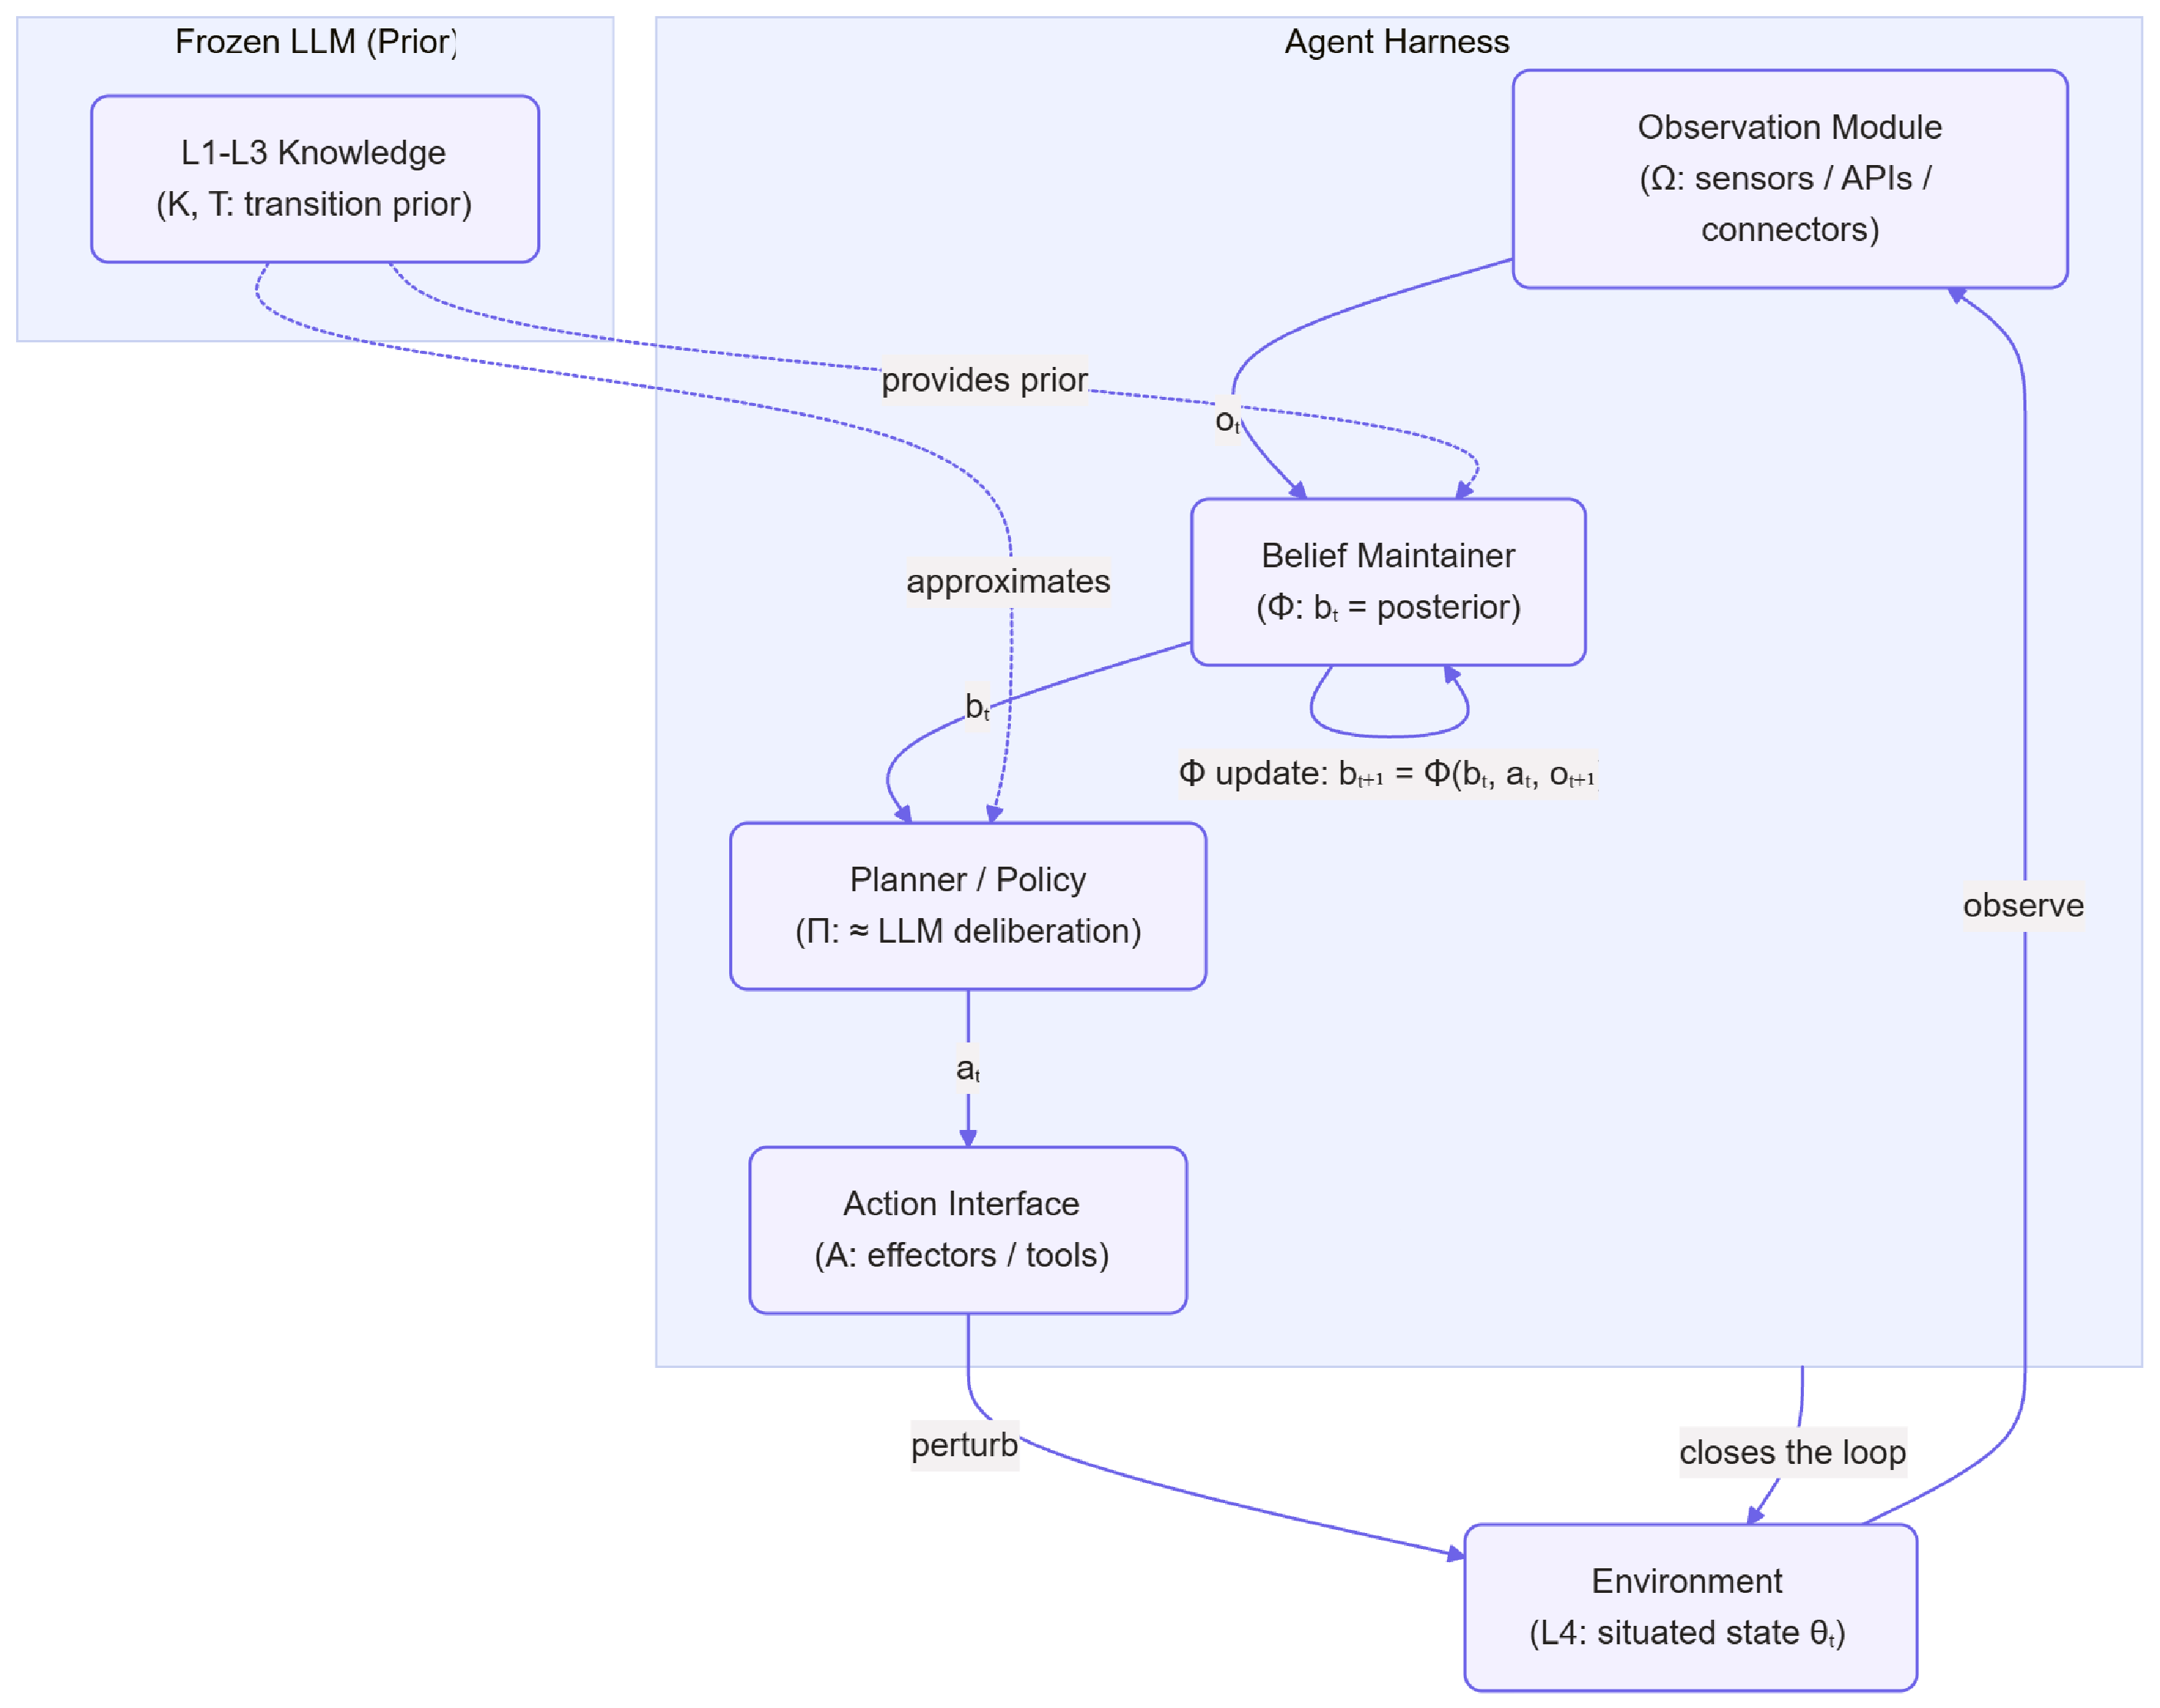
\includegraphics[width=0.85\textwidth]{figures/harness-architecture.pdf}
    \caption{The Agent Harness architecture. The frozen LLM provides \(\mathcal{K}\) and \(\mathcal{T}\); the Harness supplies \(\Omega\), \(\Phi\), and \(\Pi\). Solid arrows: data flow; dashed arrows: prior provision.}
    \label{fig:harness}
\end{figure*}
% 图：智能体框架架构。冻结LLM提供\(\mathcal{K}\)和\(\mathcal{T}\)；框架提供\(\Omega\)、\(\Phi\)和\(\Pi\)。实线箭头：数据流；虚线箭头：先验供给。

\subsection{Formalizing the Harness Architecture}

The Harness is a tuple:
\begin{equation}
\mathcal{H} = (\mathcal{S}, \mathcal{O}, \mathcal{A}, \mathcal{B}, \mathcal{T}, \Omega, \Pi),
\end{equation}
where each component corresponds to a concrete computational module:
% 框架定义为一个七元组，每个组件对应一个具体的计算模块：

\begin{itemize}
\item \(\mathcal{S} \subseteq \mathbb{R}^n\): the space of L4 environmental states \(\theta_t\), acted upon through effectors but not observed directly.
% \(\mathcal{S} \subseteq \mathbb{R}^n\)：L4环境状态\(\theta_t\)的空间，通过执行器作用于其上，但不直接观测。

\item \(\mathcal{O} \subseteq \mathbb{R}^m\): the observation space, comprising all possible observations \(o_t\) from observation modules.
% \(\mathcal{O} \subseteq \mathbb{R}^m\)：观测空间，包含来自观测模块的所有可能观测\(o_t\)。

\item \(\mathcal{A} \subseteq \mathbb{R}^k\): the action space available to the agent, instantiated through effectors.
% \(\mathcal{A} \subseteq \mathbb{R}^k\)：智能体可用的动作空间，通过执行器实例化。

\item \(\mathcal{B} \subseteq \Delta(\mathcal{S})\): the belief space, where \(b_t(\theta) = p(\theta_t \mid o_{1:t}, a_{1:t-1}, \mathcal{K})\) is the maintained posterior over L4 states.
% \(\mathcal{B} \subseteq \Delta(\mathcal{S})\)：信念空间，其中\(b_t(\theta) = p(\theta_t \mid o_{1:t}, a_{1:t-1}, \mathcal{K})\)是维护的L4状态后验。

\item \(\mathcal{T}: \mathcal{S} \times \mathcal{A} \to \Delta(\mathcal{S})\): the transition kernel
\begin{equation}
\mathcal{T}(\theta_{t+1} \mid \theta_t, a_t) = p(\theta_{t+1} \mid \theta_t, a_t, \mathcal{K}),
\end{equation}
representing the LLM's learned prior over dynamics.
% \(\mathcal{T}: \mathcal{S} \times \mathcal{A} \to \Delta(\mathcal{S})\)：转移核，表示LLM学习的动态先验。

\item \(\Omega: \mathcal{S} \to \Delta(\mathcal{O})\): the observation likelihood
\begin{equation}
\Omega(o_t \mid \theta_t) = \tilde{p}(o_t \mid \theta_t),
\end{equation}
implemented by external observation modules that transduce L4 states into textual observations.
% \(\Omega: \mathcal{S} \to \Delta(\mathcal{O})\)：观测似然，由外部观测模块实现，将L4状态转换为文本观测。

\item \(\Pi: \mathcal{B} \times \mathcal{G} \to \Delta(\mathcal{A})\): the policy/planner
\begin{equation}
\Pi(b_t, G) \approx \arg\min_{a \in \mathcal{A}} \mathbb{E}_{b_t}[\mathcal{C}(\theta, a) + \gamma V(b_{t+1})],
\end{equation}
approximated by the LLM through iterative deliberation, where \(\mathcal{G}\) is the goal space and \(\mathcal{C}\) encodes task and safety constraints.
% \(\Pi: \mathcal{B} \times \mathcal{G} \to \Delta(\mathcal{A})\)：策略/规划器，由LLM通过迭代推理近似，其中\(\mathcal{G}\)为目标空间，\(\mathcal{C}\)编码任务和安全约束。
\end{itemize}

Crucially, \(\Omega\) is not implemented by the LLM's parameters. It is supplied by external modules---sensors, APIs, or connectors---that transduce L4 into text. The grounding gap is structurally bounded by the fidelity of \(\Omega\), a constraint that scaling cannot alleviate.
% 关键在于，\(\Omega\)并非由LLM的参数实现，而是由外部模块（传感器、API或连接器）提供，将L4转译为文本。落地鸿沟在结构上受\(\Omega\)的保真度约束，这是缩放所无法缓解的。

\subsection{The Closed-Loop Dynamics}

The Harness operates as a discrete-time belief-state transition. The LLM provides \(\mathcal{T}\) and approximates \(\Pi\). But the posterior \(b_t(\theta)\) cannot be formed without \(\Omega\) and the recursive belief update \(\Phi\).
% 框架以离散时间信念状态转移的方式运作。LLM提供\(\mathcal{T}\)并近似\(\Pi\)。但后验\(b_t(\theta)\)缺少\(\Omega\)和递归信念更新\(\Phi\)则无法形成。

The loop operates in three stages:
% 环路分三个阶段运作：

\begin{enumerate}
\item \emph{Observation}: senses \(\theta_t\) and produces \(o_t\), implementing \(\Omega(o_t \mid \theta_t)\).
% \emph{观测}：感知\(\theta_t\)并产生\(o_t\)，实现\(\Omega(o_t \mid \theta_t)\)。

\item \emph{Belief update}: applies the Bayes filter \(\Phi\):
\begin{equation}
\begin{split}
b_{t+1} &= \Phi(b_t, a_t, o_{t+1}), \\
\Phi(b_t, a_t, o_{t+1})(\theta) &\propto \Omega(o_{t+1} \mid \theta) \\
&\quad \times \int_{\mathcal{S}} \mathcal{T}(\theta \mid \theta', a_t) \, b_t(\theta') \, d\theta'.
\end{split}
\end{equation}
% \emph{信念更新}：应用贝叶斯滤波器\(\Phi\)。后验正比于观测似然与预测信念的乘积。

\item \emph{Planning \& execution}: queries the LLM for \(\Pi(b_t, G)\) to produce \(a_t\), applies it via effectors, observes \(o_{t+1}\), and feeds back, closing \(b_t \to a_t \to o_{t+1} \to b_{t+1}\).
% \emph{规划与执行}：查询LLM获得\(\Pi(b_t, G)\)产生\(a_t\)，通过执行器施加，观测\(o_{t+1}\)并反馈，闭合环路\(b_t \to a_t \to o_{t+1} \to b_{t+1}\)。
\end{enumerate}

The Harness \emph{enacts} grounding, not merely accelerates it. Grounding is emergent from the coupled system.
% 框架\emph{施行}落地而非仅\emph{加速}落地。落地是耦合系统的涌现属性。

\subsection{The Harness as a Diagnostic Framework}

The tuple \(\mathcal{H}\) provides a precise vocabulary for diagnosing any LLM-based agent. For any system, we ask:
% 七元组\(\mathcal{H}\)为诊断任何基于LLM的智能体提供了精确术语。对于任何系统，我们问：

\begin{itemize}
\item Does it implement \(\Omega\) with sufficient fidelity \(\| \tilde{p} - p_{\text{real}} \|\) to track L4 dynamics?
% 是否以足够保真度\(\| \tilde{p} - p_{\text{real}} \|\)实现了\(\Omega\)以追踪L4动态？

\item Does it maintain \(b_t\) as a structured belief state updated via \(\Phi\) after each observation?
% 是否将\(b_t\)维护为通过\(\Phi\)在每次观测后更新的结构化信念状态？

\item Does it approximate \(\Pi\) using the LLM's offline knowledge and execute \(a_t\) through a causal interface?
% 是否利用LLM的离线知识近似\(\Pi\)并通过因果接口执行\(a_t\)？
\end{itemize}

L1--L3 coverage is evidenced by syntactic, physical, and factual reasoning---most current agents pass. L4 coverage, however, is evidenced only by the presence and fidelity of \(\Omega\) and \(\Phi\). By this measure, current systems cover L4 poorly, explaining their brittleness. Progress requires better Harnesses, not just better LLMs.
% L1-L3覆盖由句法、物理和事实推理证明——大多数当前智能体能通过。但L4覆盖只能由\(\Omega\)和\(\Phi\)的存在及其保真度证明。按此标准，当前系统对L4覆盖薄弱，这解释了它们的脆弱性。进步需要更好的框架，而不仅仅是更好的LLM。

The architecture is domain-general. For discrete L4 domains (e.g., DOM trees), the same framework applies with \(\mathcal{S}\) re-interpreted as a discrete state space. Two instantiations illustrate:
% 该架构是领域通用的。对于离散L4领域（如DOM树），同一框架在将\(\mathcal{S}\)重新解释为离散状态空间后仍然适用。两种实例化说明：

\begin{itemize}
\item \textbf{Physical agent} (robotics): \(\Omega\): cameras, LIDAR; \(\mathcal{A}\): motors, grippers. L4: positions, forces, occlusions.
% \textbf{物理智能体}（机器人）：\(\Omega\)：相机、激光雷达；\(\mathcal{A}\)：电机、夹爪。L4：位置、力、遮挡。

\item \textbf{Digital agent} (browser automation): \(\Omega\): DOM APIs, screenshot parsing; \(\mathcal{A}\): click, type, navigate. L4: DOM structure, application state.
% \textbf{数字智能体}（浏览器自动化）：\(\Omega\)：DOM API、截图解析；\(\mathcal{A}\)：点击、输入、导航。L4：DOM结构、应用状态。
\end{itemize}

In each case, the LLM provides \(\mathcal{T}\) and approximates \(\Pi\); the Harness supplies domain-specific \(\Omega\) and execution. The grounding problem is structurally identical across domains.
% 在每种情况下，LLM提供\(\mathcal{T}\)并近似\(\Pi\)；框架提供领域特定的\(\Omega\)和执行。落地问题在不同领域间结构上相同。

\subsection{Empirical Validation}

We instantiate the Harness on a code agent benchmark (158 EDA scripting tasks requiring correct pyAether API calls) to test our central claim: grounding gains come from \(\Omega\) fidelity, not model scale. We fix the LLM (DeepSeek-V4) and vary only the observation channel. Low-fidelity \(\Omega_{\text{vec}}\) uses name-only embedding; high-fidelity \(\Omega_{\text{hybrid}}\) combines name embedding, BM25 over descriptions, abbreviation expansion, and synonym redirect.
% 我们在一项代码智能体基准测试（158个EDA脚本任务，要求正确调用pyAether API）上实例化了该框架，以检验核心主张：落地增益来自\(\Omega\)保真度而非模型规模。固定LLM（DeepSeek-V4），仅改变观测通道。低保真\(\Omega_{\text{vec}}\)仅使用名称嵌入；高保真\(\Omega_{\text{hybrid}}\)结合名称嵌入、描述BM25、缩写展开和同义词重定向。

\begin{table*}[t]
\centering
\caption{Pass rate on 158 EDA tasks with fixed LLM, varying \(\Omega\) fidelity.}
\label{tab:omega}
\begin{tabular}{lcc}
\toprule
Configuration & \(\Omega\) Fidelity & Pass Rate \\
\midrule
Static prior only (no \(\Omega\)) & \(\varnothing\) & 0.0\% \\
Low-fidelity \(\Omega_{\text{vec}}\) & name-only & 59.5\% \\
High-fidelity \(\Omega_{\text{hybrid}}\) & name + desc + BM25 + abbrev & 87.3\% \\
\bottomrule
\end{tabular}
\end{table*}
% 表：158个EDA任务通过率，固定LLM，变化\(\Omega\)保真度。

Table~\ref{tab:omega} shows the results. With no runtime observation, pass rate is 0\%. With \(\Omega_{\text{vec}}\), it reaches 59.5\%. With \(\Omega_{\text{hybrid}}\), it improves to 87.3\%---a 27.8 percentage point gain from observation design alone, with the LLM unchanged. Over 20 Harness iterations on this benchmark, pass rate evolved from 59.5\% to 91.1\% without any model change, supporting our claim that environmental adaptation is achieved through observation and action channel design, not parameter tuning.
% 表~\ref{tab:omega}展示了结果。无运行时观测时通过率为0\%。\(\Omega_{\text{vec}}\)下为59.5\%。\(\Omega_{\text{hybrid}}\)下提升至87.3\%——仅通过观测设计就获得27.8个百分点增益，LLM不变。在该基准上经过20多次框架迭代，通过率从59.5\%演进至91.1\%，未改变任何模型，支持了我们的主张：环境适应通过观测和动作通道设计实现，而非参数调优。

\subsection{Design Principles}

The formalization yields three architectural principles:
% 上述形式化产生三条架构原则：

\begin{enumerate}
\item \emph{Closed-loop necessity}: The observation-action loop must be continuous; \(\Phi\)'s update rate must exceed the characteristic timescale of L4 dynamics.
% \emph{闭环必要性}：观测-动作环路必须持续；\(\Phi\)的更新率必须超过L4动态的特征时间尺度。

\item \emph{Observation fidelity}: Minimize \(\| \tilde{p} - p_{\text{real}} \|\) by optimizing observation modules. Information lost in \(\Omega\) cannot be recovered by a larger LLM.
% \emph{观测保真度}：通过优化观测模块最小化\(\| \tilde{p} - p_{\text{real}} \|\)。\(\Omega\)中丢失的信息无法由更大的LLM恢复。

\item \emph{Belief maintenance}: Maintain \(b_t\) as a structured representation capturing uncertainty and history, enabling recovery from unexpected changes.
% \emph{信念维护}：将\(b_t\)维护为捕获不确定性和历史的结构化表征，使其能从意外变化中恢复。
\end{enumerate}
\section{Design Principles for Grounded Agents}

The Harness formalization in Section 5 yields three architectural principles that form a coherent thesis: freeze knowledge $\mathcal{K}$, maximize observation $\Omega$, and run belief update $\Phi$ continuously. Training changes $\mathcal{K}$; observation changes belief $b_t$; action changes the environment. The system adapts through belief, not parameter updates.
% 第5节的框架形式化产生三条架构原则，它们构成一个连贯的论点：冻结知识$\mathcal{K}$、最大化观测$\Omega$、持续运行信念更新$\Phi$。训练改变$\mathcal{K}$；观测改变信念$b_t$；行动改变环境。系统通过信念而非参数更新来适应。

\subsection{Decouple Knowledge from Belief}

Knowledge $\mathcal{K}$ is the static L1--L3 prior encoded in the LLM's parameters---general, context-free, derived from text. Belief $b_t(\theta) = p(\theta_t \mid o_{1:t}, a_{1:t-1}, \mathcal{K})$ is the dynamic posterior maintained by the Harness---specific, context-dependent, updated via $\Phi$ with each observation.
% 知识$\mathcal{K}$是LLM参数中编码的静态L1--L3先验——通用的、上下文无关的、来源于文本。信念$b_t(\theta) = p(\theta_t \mid o_{1:t}, a_{1:t-1}, \mathcal{K})$是框架维护的动态后验——特定的、上下文依赖的、通过$\Phi$随每次观测更新。

Fine-tuning the LLM during deployment attempts to update $\mathcal{K}$ with limited local observations---inefficient and risks catastrophic forgetting. Instead, freeze $\mathcal{K}$; absorb all adaptation in $b_t$. This separation yields stability (prior robust across tasks) and flexibility (belief tracks the current state) simultaneously.
% 部署期间微调LLM试图用有限的局部观测更新$\mathcal{K}$——低效且有灾难性遗忘风险。相反，冻结$\mathcal{K}$；将所有适应吸收在$b_t$中。这种分离同时实现了稳定性（先验跨任务稳健）和灵活性（信念跟踪当前状态）。

\subsection{Optimize Observation Over the Prior}

The scaling debate has focused overwhelmingly on the prior. But the formalization reveals a structural asymmetry: the grounding gap is bounded by the \emph{fidelity of the likelihood} $\Omega$, not by the expressiveness of the prior $\mathcal{T}$. As established in Section 4, $D_{\text{grounding}}(t)$ is bounded by $\|\tilde{p} - p_{\text{real}}\|$---a bound independent of model scale.
% 缩放争论已压倒性地聚焦于先验。但形式化揭示了一个结构不对称：落地鸿沟被似然$\Omega$的\emph{保真度}所界定，而非被先验$\mathcal{T}$的表达能力所界定。如第4节所述，$D_{\text{grounding}}(t)$被$\|\tilde{p} - p_{\text{real}}\|$所界定——该上界与模型规模无关。

Investment in observation---sensors, APIs, connectors, state estimators---has a direct, bounded effect on performance. Investment in model scale, once the prior is sufficiently rich, has diminishing returns: it cannot reduce the grounding gap below the observation-imposed floor.
% 对观测的投入——传感器、API、连接器、状态估计器——对性能有直接的、有界的效应。一旦先验足够丰富，对模型规模的投入收益递减：它无法将落地鸿沟降低到观测所施加的下限以下。

\subsection{Design for Continuous Belief Updating}

Belief update $\Phi$ operates online: every observation $o_t$ yields a recursive update $b_t \mapsto b_{t+1}$. This fundamentally differs from the static training-then-deploy paradigm. In dynamic L4 environments, the system must update with every observation.
% 信念更新$\Phi$在线运作：每次观测$o_t$产生递归更新$b_t \mapsto b_{t+1}$。这根本不同于静态的"训练-部署"范式。在动态L4环境中，系统必须在每次观测时更新。

Two implications follow. First, $\Phi$'s update rate must exceed the timescale of L4 dynamics; otherwise $b_t$ becomes stale. Second, $b_t$ must be a structured representation that captures uncertainty and history, enabling recovery from unexpected changes and reasoning under partial observability. (Filtering methods such as particle filters or Kalman filters are familiar instantiations of this principle, but the framework itself does not depend on any particular implementation.)
% 两个含义：第一，$\Phi$的更新率必须超过L4动态的时间尺度；否则$b_t$会过时。第二，$b_t$必须是一个结构化的表征，捕获不确定性和历史，使其能够从意外变化中恢复并在部分可观测下推理。（粒子滤波器或卡尔曼滤波器等滤波方法是这一原则的常见实例化，但框架本身并不依赖任何特定实现。）

Together, these three principles form a coherent architecture: freeze $\mathcal{K}$, maximize $\Omega$, run $\Phi$ continuously. The Harness operationalizes all three.
% 这三条原则共同构成一个连贯的架构：冻结$\mathcal{K}$、最大化$\Omega$、持续运行$\Phi$。框架将所有三者操作化。
\section{Alternative Views}

A counter-position to our thesis holds that scaling---larger models, broader pretraining corpora, and more sophisticated world models---can eventually render runtime observation unnecessary. According to this view, L4 states are not fundamentally different from L1--L3; they are merely high-dimensional, fine-grained historical facts that a sufficiently powerful prior can approximate. If the prior captures enough of the world's dynamics, the argument goes, prediction from the prior may suffice for action, eliminating the need for real-time observation.
% 与我们论点相对的一个立场认为，规模扩展——更大的模型、更广泛的预训练语料和更精密的世界模型——最终可以使运行时观测变得不必要。根据这一观点，L4状态与L1--L3在根本上并无不同；它们仅仅是高维的、细粒度的历史事实，一个足够强大的先验可以近似它们。如果先验捕捉了足够多的世界动态，论证认为，从先验出发的预测可能就足以指导行动，从而消除了实时观测的需要。

We reject this view on three grounds. First, L4 states are \emph{indexical} by definition: they depend on \emph{when} and \emph{where} the agent is. A prior learned from past data cannot, by construction, guarantee facts about the current state that came into existence after the training cutoff. No amount of scaling can compress information that does not yet exist at training time. Second, the exponential growth of possible L4 configurations means that any finite prior will be sparse in the space of actual situated states. The agent will inevitably encounter configurations not represented in its training distribution. Third, even a perfect prior is still a distribution over states, not a certificate of the actual state. Grounding requires contact with the environment, not just probabilistic inference from memory.
% 我们基于三点理由拒绝这一观点。第一，L4状态按其定义是\emph{指示性}的：它们取决于智能体所在的\emph{何时}与\emph{何地}。从过去数据中学习的先验在构造上无法保证关于训练截止日期之后才出现的当前状态的事实。无论规模多大，都无法压缩训练时尚不存在的信息。第二，可能的L4配置呈指数增长，意味着任何有限先验在实际情境状态空间中都是稀疏的。智能体将不可避免地遇到其训练分布中未表示的配置。第三，即使是完美的先验，也仍然是状态上的分布，而非实际状态的证明。落地需要与环境接触，而不仅仅是从记忆中进行概率推理。

An alternative position might propose that embodied interaction with the environment can be folded into the LLM itself through online fine-tuning or continual learning, eliminating the need for a separate Harness architecture.
% 另一种替代立场可能提出，通过与环境的具身交互可以通过在线微调或持续学习融入LLM本身，从而消除对独立框架架构的需求。

We acknowledge that end-to-end online adaptation is an active research direction. However, our framework does not claim that the Harness is the \emph{only} possible architecture; it claims that for \emph{current} text-trained, frozen-parameter LLMs, a runtime Harness is structurally necessary. For future architectures that learn primarily through online interaction, the boundary between \(\mathcal{K}\) and \(b_t\) may shift or disappear. This is a limitation we acknowledge in Section~9.1. Our contribution is a diagnostic framework for \emph{current} systems, not a universal claim about all possible intelligent systems.
% 我们承认端到端的在线适应是一个活跃的研究方向。然而，我们的框架并不主张框架是\emph{唯一}可能的架构；它主张对于\emph{当前}的基于文本训练的、参数冻结的LLM，运行时框架在结构上是必要的。对于主要通过在线交互学习的未来架构，\(\mathcal{K}\)与\(b_t\)之间的边界可能移动或消失。这是我们在第9.1节中承认的一个局限。我们的贡献是面向\emph{当前}系统的诊断框架，而非关于所有可能智能系统的普遍主张。
\section{Call to Action}

The Grounding Gap is not an inevitable property of all AI systems; it is a design choice embedded in the current paradigm of static, offline-trained models. Addressing it requires coordinated action from three communities.
% 落地鸿沟并非所有AI系统的必然属性；它是嵌入在当前静态、离线训练模型范式中的一种设计选择。解决它需要来自三个群体的协调行动。

\textbf{Researchers:} Shift evaluation focus from model-centric benchmarks to system-level diagnostics. Measure not just what the model knows (L1--L3), but how well the system observes L4 states and maintains belief over time. The three diagnostic questions in Section~5.3 provide a starting framework.
% \textbf{研究者：}将评估焦点从以模型为中心的基准转向系统级诊断。不仅衡量模型知道什么（L1--L3），还要衡量系统观测L4状态并随时间维护信念的能力。第5.3节中的三个诊断性问题提供了一个起始框架。

\textbf{System architects:} Build Harnesses as first-class components, not afterthoughts. \(\Omega\) (observation) and \(\Phi\) (belief update) should be designed with the same rigor as the LLM itself. Prioritize observation fidelity---sensors, APIs, connectors---over model scale once the prior is sufficiently rich.
% \textbf{系统架构师：}将框架作为一等组件来构建，而非事后的补丁。\(\Omega\)（观测）和\(\Phi\)（信念更新）应以与LLM本身相同的严谨程度来设计。一旦先验足够丰富，应将观测保真度——传感器、API、连接器——置于模型规模之上。

\textbf{Community:} Develop shared benchmarks and protocols for evaluating grounded agents. Current benchmarks test static reasoning; we need benchmarks that require real-time observation, belief maintenance, and recovery from unexpected changes. Such benchmarks would make the Grounding Gap measurable and progress accountable.
% \textbf{社区：}开发用于评估落地智能体的共享基准和协议。当前基准测试静态推理；我们需要要求实时观测、信念维护和从意外变化中恢复的基准。这样的基准将使落地鸿沟可衡量，使进展可问责。

The shift from larger static artifacts to dynamic, situated systems is not a technological inevitability---it is a choice. The sooner we make it, the sooner agentic AI will move from impressive demos to reliable action in the real world.
% 从更大的静态制品向动态、情境化系统的转变并非技术的必然——它是一种选择。我们越早做出这一选择，行动AI就能越早从令人印象深刻的演示走向现实世界中的可靠行动。
\section{Limitations}

Our framework rests on several assumptions that bound its scope.
% 我们的框架依赖于若干限制其适用范围的假设。

\subsection{Knowledge--Belief Separation}

The separation between $\mathcal{K}$ and $b_t$ is analytically useful but not metaphysically necessary. End-to-end architectures that adapt online may blur this boundary. Our framework is a pragmatic carving for text-trained models deployed in dynamic environments, not a claim about all possible intelligent systems. For future architectures that learn primarily through interaction---embodied foundation models trained online---this boundary may shift or disappear.
% $\mathcal{K}$与$b_t$的分离在分析上有用，但并非形而上学上的必然。在线适应的端到端架构可能模糊这一边界。我们的框架是针对在动态环境中部署的文本训练模型的实用划分，而非对所有可能智能系统的论断。对于主要通过交互学习的未来架构——在线训练的具身基础模型——这一边界可能移动或消失。

\subsection{Transition Kernel Imperfections}

The framework assumes a well-defined transition kernel $\mathcal{T}$ supplied by the LLM. In practice, $\mathcal{T}$ is implicit and may hallucinate; $\Omega$ can correct this only as reliably as observation permits. When the LLM's physical or causal reasoning is flawed, $b_t$ inherits that error. The Harness can mitigate this through frequent observation resets and conservative planning, but cannot eliminate errors that the prior systematically encodes. Our bounds on the grounding gap assume $\mathcal{T}$ is fixed and correct in its support---relaxing this assumption is future work.
% 该框架假设LLM提供了良好定义的转移核$\mathcal{T}$。实践中$\mathcal{T}$是隐式的且可能产生幻觉；$\Omega$的纠正仅取决于观测的可靠性。当LLM的物理或因果推理存在缺陷时，$b_t$继承该误差。框架可通过频繁观测重置和保守规划缓解，但无法消除先验系统性编码的误差。我们对落地鸿沟的界假设$\mathcal{T}$在其支撑集上固定且正确——放松这一假设是未来工作。

\subsection{Approximate Belief Updating}

Exact Bayesian inference via $\Phi$ is intractable in high-dimensional $\mathcal{S}$; every implementation must approximate it, and the framework does not bound this approximation error. Approximate implementations of $\Phi$---such as the filtering methods noted in Section~6.3---introduce approximation error, and its interaction with the LLM's prior is not fully understood. The framework provides a conceptual formalization for diagnosis and architecture design, not a directly implementable algorithm with provable performance guarantees.
% 高维$\mathcal{S}$中通过$\Phi$的精确贝叶斯推断是棘手的；每个实现都必须近似，框架未界定近似误差。$\Phi$的近似实现（如第6.3节提及的滤波方法）会引入近似误差，其与LLM先验的相互作用尚未被充分理解。该框架提供了用于诊断和架构设计的概念性形式化，而非带有可证明性能保证的直接可实现算法。

\subsection{Practical Scope}

The framework is not a complete agent implementation. It abstracts away plan generation, cost specification, and domain-specific state distinctions---not as oversights, but as intentional scope delimiters. The four-level distinction and Bayesian engine operate above these details; they are scaffolding for diagnosis and architecture design, not a turnkey system. Applying the framework to a particular domain requires instantiating $\mathcal{A}$, $\mathcal{C}$, and the relevant L4 state space, all of which are domain-dependent and deliberately left unspecified.
% 该框架并非一个完整的智能体实现。它抽象掉了计划生成、成本函数具体化以及领域特定的状态区分——这些不是疏忽，而是有意的范围界定。四层区分和贝叶斯引擎在这些细节之上运作；它们是用作诊断和架构设计的脚手架，而非拿来即用的系统。将框架应用于特定领域需要实例化$\mathcal{A}$、$\mathcal{C}$以及相关的L4状态空间，这些均是领域依赖的，且有意识地未做具体规定。
\section{Conclusion}

The paradox that opened this paper is not a knowledge deficit but a structural consequence: an LLM is a static compressor of what has been written, blind to what is happening now. The grounding gap is the distance between offline knowledge (L1--L3) and situated truth (L4). L4 is indexical, ephemeral, and cannot be learned from static text. It must enter through runtime observation, not pretraining. This distinction---recalling what was versus observing what is---is our central contribution.
% 开篇悖论并非知识匮乏，而是结构性后果：LLM是已书写内容的静态压缩器，对此刻正在发生的事情视而不见。落地鸿沟是离线知识（L1-L3）与情境真实（L4）之间的距离。L4是指示性的、瞬时性的，无法从静态文本中学习。它必须通过运行时观测而非预训练进入系统。这一区分——回忆曾经是什么与观测当前是什么——是我们的核心贡献。

To bridge this gap, we introduced the Agent Harness, formalized as \(\mathcal{H} = (\mathcal{S}, \mathcal{O}, \mathcal{A}, \mathcal{B}, \mathcal{T}, \Omega, \Pi)\). The LLM provides the learned prior \(\mathcal{T}\) and approximates planning; the Harness supplies runtime observation \(\Omega\), belief update \(\Phi\), and execution. The central insight: the grounding gap is bounded by the fidelity of \(\Omega\), not by the capacity of \(\mathcal{T}\). Scaling improves the prior but cannot compensate for a lossy observation channel.
% 为弥合这一鸿沟，我们引入了智能体框架，形式化为\(\mathcal{H} = (\mathcal{S}, \mathcal{O}, \mathcal{A}, \mathcal{B}, \mathcal{T}, \Omega, \Pi)\)。LLM提供学习先验\(\mathcal{T}\)并近似规划；框架提供运行时观测\(\Omega\)、信念更新\(\Phi\)和执行。核心洞见：落地鸿沟受\(\Omega\)保真度约束，而非\(\mathcal{T}\)的容量。缩放改进了先验，但无法补偿有损的观测通道。

Three principles follow: freeze \(\mathcal{K}\), maximize \(\Omega\), run \(\Phi\) continuously. These shift the field from building larger static artifacts to designing dynamic real-time systems. Training changes knowledge; observation changes belief; action changes the world.
% 三条原则由此推出：冻结\(\mathcal{K}\)、最大化\(\Omega\)、持续运行\(\Phi\)。它们将领域从构建更大的静态制品转向设计动态的实时系统。训练改变知识；观测改变信念；行动改变世界。

The model compresses the past; the system meets the present; situated intelligence emerges from their coupling.
% 模型压缩过去；系统面对当下；情境智能从它们的耦合中涌现。

\bibliographystyle{icml2025}
\bibliography{references}

\newpage
\appendix
\onecolumn
% \section{Appendix}

% 附录内容

\end{document}
